\section{Case Study A: OpenCL Heterogeneous Mapping}
\label{sec:deeptune-case-study-a}

OpenCL provides a platform-agnostic framework for heterogeneous parallelism. This allows a program written in OpenCL to execute transparently across a range of different devices, from CPUs to GPUs and FPGAs. Given a program and a choice of execution devices, the question then is on which device should one execute the program to maximise performance?

\subsection{State-of-the-art}

We return to the \citeauthor{Grewe2013}~\cite{Grewe2013} predictive model of Chapter~\ref{chap:clgen} for mapping OpenCL kernels to the optimal device in CPU/GPU heterogeneous systems. They use supervised learning to construct decision trees, using a combination of static and dynamic kernel features. The static program features are extracted using a custom LLVM pass; the dynamic features are taken from the OpenCL runtime.

\paragraph*{Expert Chosen Features}

Table~\ref{tab:grewe-features-final} shows the features used in their work. Each feature is an expression built upon the code and runtime metrics given in Table~\ref{tab:grewe-features-raw}.

\begin{table}
  \rowcolors{2}{gray!25}{white}
  \centering%
  \subfloat[Feature values]{
    \begin{tabular}{| l L{4.5cm} |}
      \hline
      \rowcolor{gray!50}
      \textbf{Name} & \textbf{Description} \\
      \hline
      \texttt{F1: data size/(comp+mem)} & commun.-computation ratio \\
      \texttt{F2: coalesced/mem} & \% coalesced memory accesses \\
      \texttt{F3: (localmem/mem)$\times$wgsize} & ratio local to global mem accesses  $\times$ \#.\ work-items \\
      \texttt{F4: comp/mem} & computation-mem ratio\\
      \hline
    \end{tabular}%
    \label{tab:grewe-features-final}%
  }\\ %
  \subfloat[Values used in feature computation]{%
    \rowcolors{2}{gray!25}{white}
    \begin{tabular}{| l c l |}
    	\hline
      \rowcolor{gray!50}
      \textbf{Name} & \textbf{Type} & \textbf{Description} \\
      \hline
      \texttt{comp} & static & \#.\ compute operations \\
      \texttt{mem} & static & \#.\ accesses to global memory \\
      \texttt{localmem} & static & \#.\ accesses to local memory \\
      \texttt{coalesced} & static & \#.\ coalesced memory accesses \\
      \texttt{data size} & dynamic & size of data transfers \\
      \texttt{work-group size} & dynamic & \#.\ work-items per kernel \\
      \hline
    \end{tabular}%
    \label{tab:grewe-features-raw}%
  }
  \caption[Heterogeneous mapping model features]{%
    Features used by \emph{Grewe et al. }to predict heterogeneous device
    mappings for OpenCL kernels.%
  } %
  \label{tab:grewe-features} %
\end{table}


\subsection{Experimental Setup}

The predictive model of \citeauthor{Grewe2013}~\cite{Grewe2013} is replicated. The same experimental setup is used as in Chapter~\ref{chap:clgen} in which the experiments are extended to a larger set of 71 programs, summarised in Table~\ref{tab:cgo-benchmarks}. The programs were evaluated on two CPU-GPU platforms, detailed in Table~\ref{tab:cgo-platforms}.

\begin{table}
	\centering%
	\rowcolors{2}{gray!25}{white}
	\begin{tabular}{| l r r r |}
		\hline
		\rowcolor{gray!50}
		& \textbf{Version} & \textbf{\#. benchmarks} & \textbf{\#. kernels}\\
		\hline
		\textbf{NPB (SNU~\cite{Seo2011})} & 1.0.3 & 7 & 114 \\
		\textbf{Rodinia~\cite{Che2009}} & 3.1 & 14 & 31 \\
		\textbf{NVIDIA SDK} & 4.2 & 6 & 12 \\
		\textbf{AMD SDK} & 3.0 & 12 & 16 \\
		\textbf{Parboil~\cite{Stratton2012}} & 0.2 & 6 & 8 \\
		\textbf{PolyBench~\cite{Grauer-Gray2012}} & 1.0 & 14 & 27 \\
		\textbf{SHOC~\cite{Danalis2010}} & 1.1.5 & 12 & 48 \\
		\textbf{Total} & - & 71 & 256 \\
		\hline
	\end{tabular}
  \caption[Benchmarks used in Case Study A]{%
	  Benchmarks used in Case Study A.%
  }
	\label{tab:cgo-benchmarks}
\end{table}

\begin{table}[t!]
	\centering %
		\rowcolors{2}{gray!25}{white}
		\begin{tabular}{| l l l l| }
			\hline
			\rowcolor{gray!50}
			& \textbf{Frequency} & \textbf{Memory} & \textbf{Driver} \\
			\hline
			\textbf{Intel Core i7-3820} & 3.6 GHz & 8GB & AMD 1526.3 \\
			\textbf{AMD Tahiti 7970} & 1000 MHz & 3GB & AMD 1526.3 \\
			\textbf{NVIDIA GTX 970} & 1050 MHz & 4GB & NVIDIA 361.42 \\
			\hline
		\end{tabular}
	  \caption[Benchmarks used in Case Study A]{%
		Experimental platforms used in Case Study A.%
  	}
		\label{tab:cgo-platforms}
\end{table}


\paragraph*{DeepTune Configuration}

Figure~\ref{fig:nn}a shows the neural network configuration of DeepTune for the task of predicting optimal device mapping. The OpenCL kernel source code is used as input, along with the two dynamic values \emph{work-group size} and \emph{data size} available to the OpenCL runtime.

\paragraph*{Model Evaluation}

\emph{Stratified 10-fold cross-validation} is used to evaluate the quality of the predictive models~\cite{Han2011}. Each program is randomly allocated into one of 10 equally-sized sets; the sets are balanced to maintain a distribution of instances from each class consistent with the full set. A model is trained on the programs from all but one of the sets, then tested on the programs of the unseen set. This process is repeated for each of the 10 sets, to construct a complete prediction over the whole data set.

\begin{figure}[t!]
  \centering
  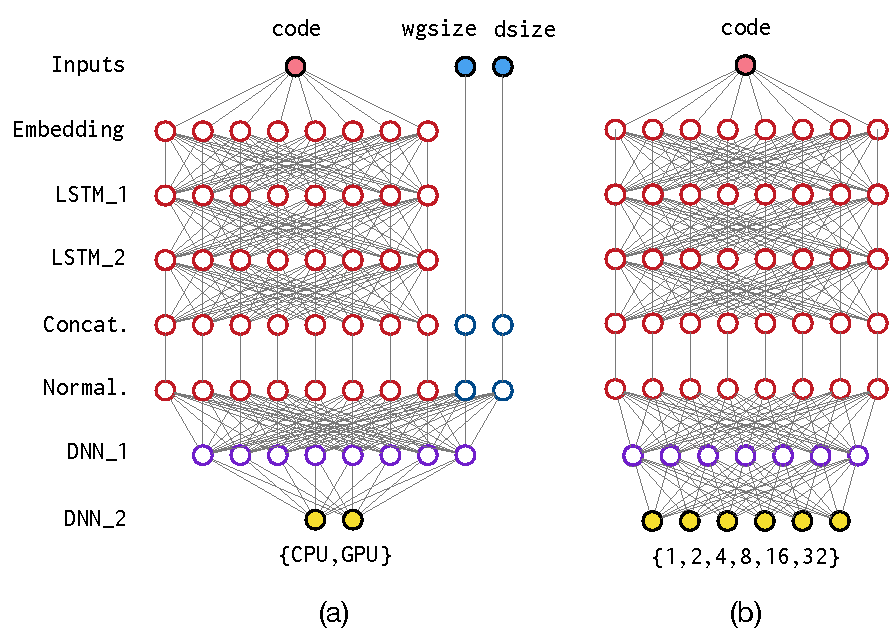
\includegraphics[width=\columnwidth]{img/nn} %
  \caption[DeepTune artificial neural networks]{%
    DeepTune artificial neural networks, configured for (a) heterogeneous mapping, and (b) thread coarsening factor. The design stays almost the same regardless of the optimisation problem. The only changes are the extra input for (a) and size of the output layers.%
  }%
  \label{fig:nn}
\end{figure}



\subsection{Experimental Results}

Selecting the optimal execution device for OpenCL kernels is essential for maximising performance. For a CPU/GPU heterogeneous system, this presents a binary choice. In this experiment, the approach is compared against a static single-device approach and the \citeauthor{Grewe2013} predictive model. The \emph{static mapping} selects the device which gave the best average case performance over all the programs. On the AMD platform, the best-performing device is the CPU; on the NVIDIA platform, it is the GPU.

Figure~\ref{fig:cgo-accuracy} shows the accuracy of both predictive models and the static mapping approach for each of the benchmark suites. The static approach is accurate for only 58.8\% of cases on AMD and 56.9\% on NVIDIA. This suggests the need for choosing the execution device on a per program basis. The \citeauthor{Grewe2013} model achieves an average accuracy of 73\%, a significant improvement over the static mapping. By automatically extracting useful feature representations from the source code, DeepTune gives an average accuracy of 82\%, an improvement over both schemes.

\begin{figure}
	\centering %
	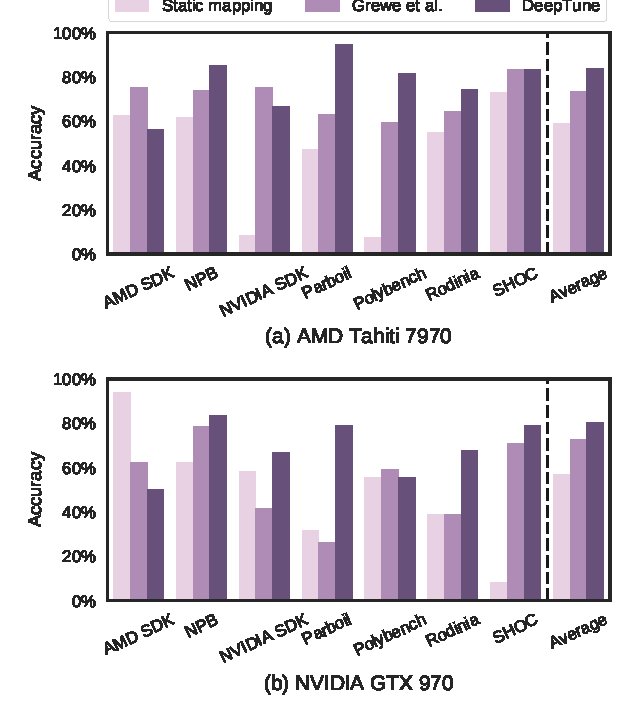
\includegraphics[width=.85\columnwidth]{img/cgo-acc}%
	\caption[Accuracy of optimisation heuristics for heterogeneous device mapping]{%
		Accuracy of optimisation heuristics for heterogeneous device mapping, aggregated by benchmark suite. The optimal static mapping achieves 58\% accuracy. The \citeauthor{Grewe2013} and DeepTune predictive models achieve accuracies of 73\% and 84\%, respectively.%
	}
	\label{fig:cgo-accuracy}
\end{figure}

Using the static mapping as a baseline, the relative performance of each program is computed using the device selected by the \citeauthor{Grewe2013} and DeepTune models. Figure~\ref{fig:cgo-speedup} shows these speedups. Both predictive models significantly outperform the static mapping; the Grewe \emph{et al.\ }model achieves an average speedup of $2.91\times$ on AMD and $1.26\times$ on NVIDIA (geometric mean $1.18\times$). In 90\% of cases, DeepTune matches or outperforms the predictions of the Grewe \emph{et al.\ }model, achieving an average speedup of $3.34\times$ on AMD and $1.41\times$ on NVIDIA (geometric mean $1.31\times$). This 14\% improvement in performance comes at a greatly reduced cost, requiring no intervention by humans.

\begin{figure}
	\centering %
	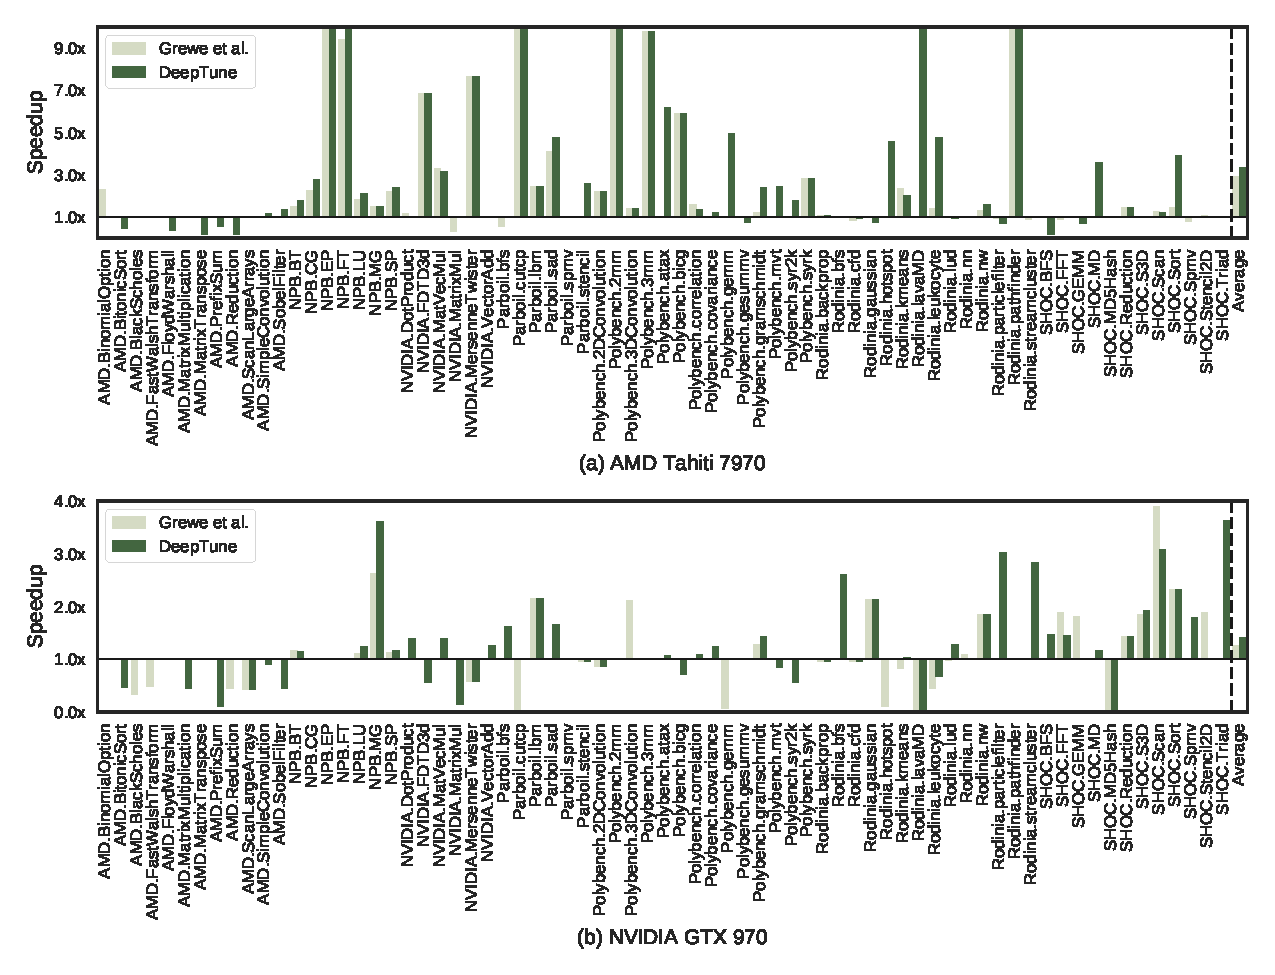
\includegraphics[width=\textwidth]{img/cgo-speedup}%
	\caption[Speedup of predicted heterogeneous mappings]{%
		Speedup of predicted heterogeneous mappings over the best static mapping for both platforms. In (a) DeepTune achieves an average speedup of 3.43x over static mapping and 18\% over \citeauthor{Grewe2013}. In (b) the speedup is 1.42x and 13\% respectively.%
	}
	\label{fig:cgo-speedup}
\end{figure}



\section{Case Study B: OpenCL Thread Coarsening Factor}
\label{sec:deeptune-case-study-b}

Thread coarsening is an optimisation for parallel programs in which the operations of two or more threads are fused together. This optimisation can prove beneficial on certain combinations of programs and architectures, for example programs with a large potential for Instruction Level Parallelism on Very Long Instruction Word architectures.

\subsection{State-of-the-art} \citeauthor{Magni2014}present a predictive model for OpenCL thread coarsening in~\cite{Magni2014}. They implement an iterative heuristic which determines whether a given program would benefit from coarsening. If yes, then the program is coarsened, and the process repeats, allowing further coarsening. In this manner, the problem is reduced from a multi-label classification problem into a series of binary decisions, shown in Figure~\ref{fig:cf-magni}. They select from one of six possible coarsening factors: $(1, 2, 4, 8, 16, 32)$, divided into 5 binary choices.

\begin{figure}
  \centering %
  \subfloat[Magni \emph{et al.\ }cascading binary model.]{%
    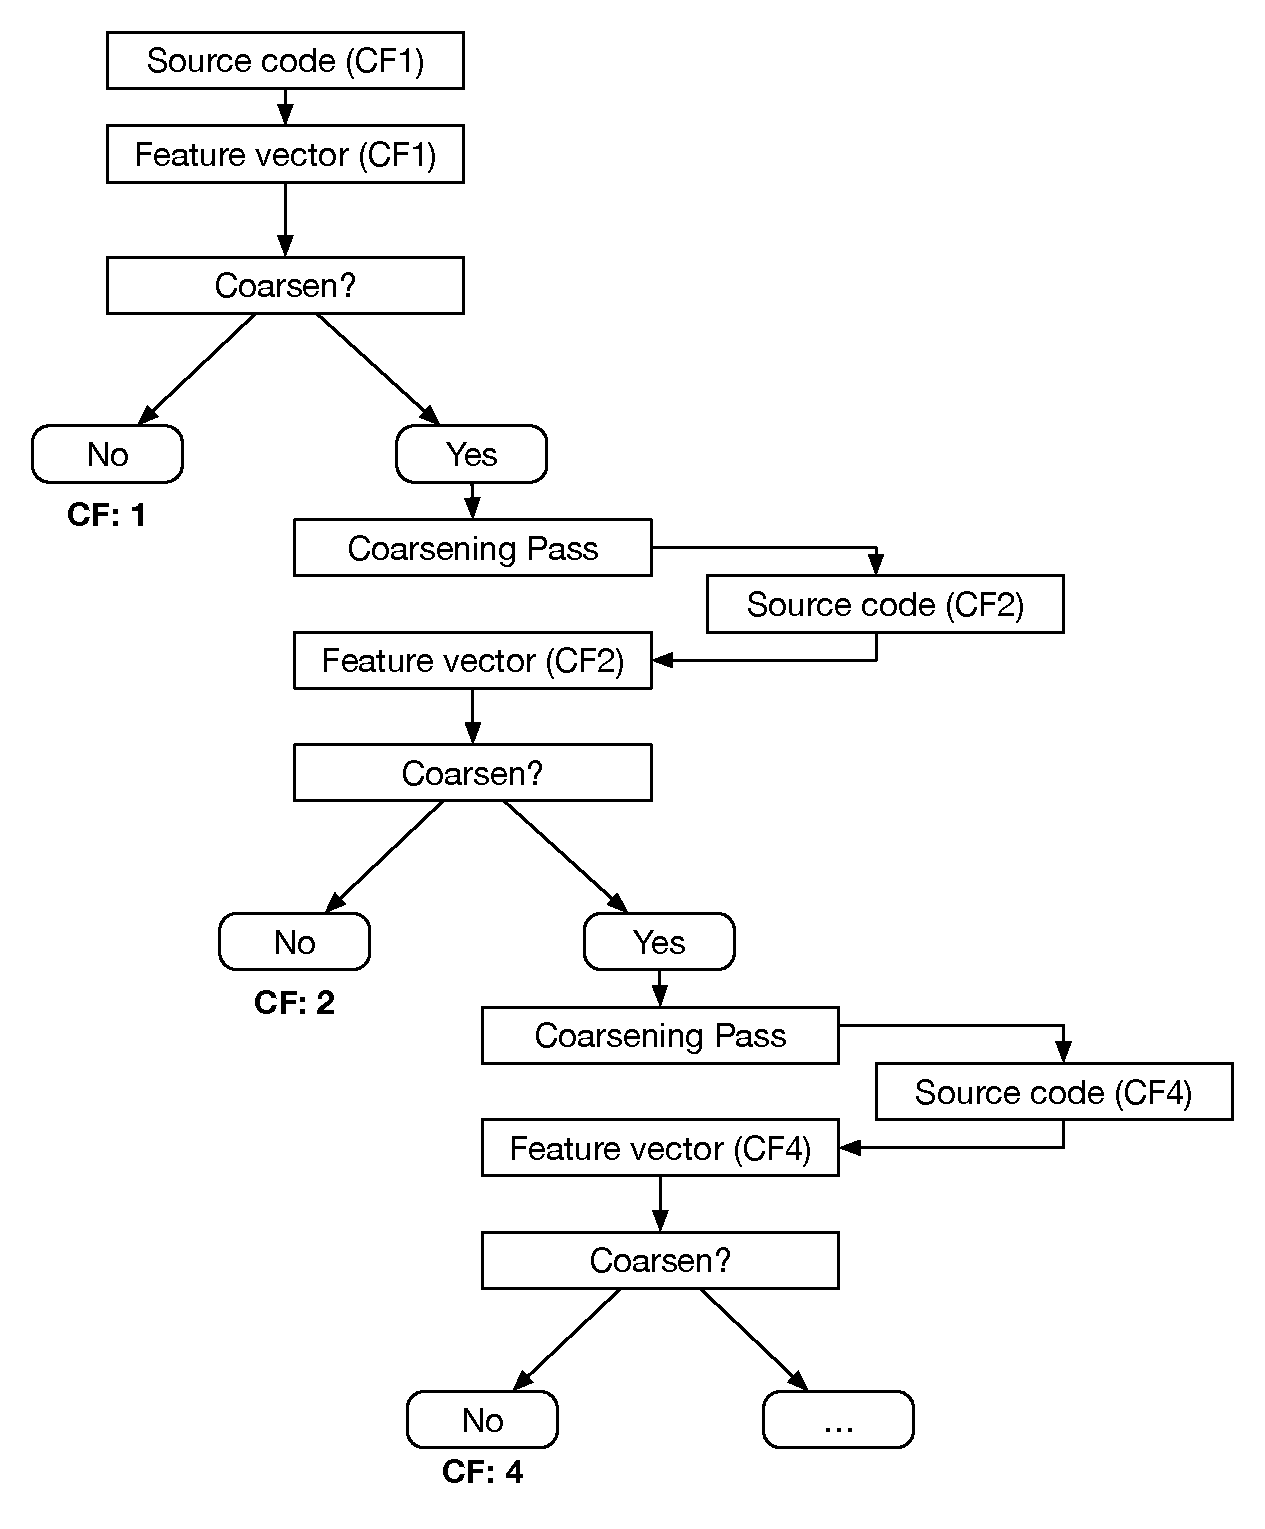
\includegraphics[width=.85\columnwidth]{img/cf-magni}%
    \label{fig:cf-magni}
  }\\*%
  \subfloat[Our approach.]{%
      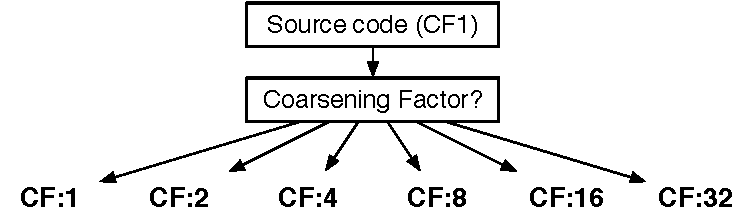
\includegraphics[width=.65\columnwidth]{img/cf-deeptune}%
      \label{fig:cf-deeptune}
  }%
  \caption{%
      Two approaches for predicting coarsening factor (CF) of OpenCL kernels.
      Magni \emph{et al.\ }reduce the multi-label classification problem to a
      series of binary decisions, by iteratively applying the optimization and
      computing new feature vectors. Our approach simply predicts the coarsening
      factor directly from the source code.%
  }
  \label{fig:cascading-nn}
\end{figure}


\begin{table}
  \rowcolors{2}{gray!25}{white}
  \centering%
    \begin{tabular}{| l l |}
      \hline
      \rowcolor{gray!50}
      \textbf{Name} & \textbf{Description} \\
      \hline
      \texttt{BasicBlocks} & \#.\ basic blocks \\
      \texttt{Branches} & \#.\ branches \\
      \texttt{DivInsts} & \#.\ divergent instructions \\
      \texttt{DivRegionInsts} & \#.\ instructions in divergent regions \\
      \texttt{DivRegionInstsRatio} & \#.\ instr. in divergent regions / total instructions \\
      \texttt{DivRegions} & \#.\ divergent regions \\
      \texttt{TotInsts} & \#.\ instructions \\
      \texttt{FPInsts} & \#.\ floating point instructions \\
      \texttt{ILP} & average ILP / basic block \\
      \texttt{Int/FP Inst Ratio} & \#.\ branches \\
      \texttt{IntInsts} & \#.\ integer instructions \\
      \texttt{MathFunctions} & \#.\ match builtin functions \\
      \texttt{MLP} & average MLP / basic block \\
      \texttt{Loads} & \#.\ loads \\
      \texttt{Stores} & \#.\ stores \\
      \texttt{UniformLoads} & \#.\ loads unaffected by coarsening direction \\
      \texttt{Barriers} & \#.\ barriers \\
      \hline
    \end{tabular}%
    \label{tab:features-pact14-raw}%
  \caption[\emph{Magni et al.\ }features for predicting thread coarsening]{%
    Candidate features used by \emph{Magni et al.\ }for predicting thread
    coarsening. From these values, they compute relative deltas for each
    iteration of coarsening, then use PCA for selection.%
  }%
  \label{tab:magni-features} %
\end{table}


\paragraph*{Expert Chosen Features}

\citeauthor{Magni2014}followed a very comprehensive feature engineering process. 17 candidate features were assembled from previous studies of performance counters and computed theoretical values~\cite{Magni2,Sim2012}. For each candidate feature they compute its coarsening \emph{delta}, reflecting the change in each feature value caused by coarsening: $f_{\Delta} = (f_{after} - f_{before}) / f_{before}$, adding it to the feature set. Then they use Principle Component Analysis (PCA) on the 34 candidates and selected the first 7 principle components, accounting for 95\% of variance in the space.

\subsection{Experimental Setup}

The experimental setup of \citeauthor{Magni2014}~\cite{Magni2014} is replicated. The thread coarsening optimisation is evaluated on 17 programs, listed in Table~\ref{tab:pact-benchmarks}. Four different GPU architectures are used, listed in Table~\ref{tab:pact-platforms}.

\begin{table}
	\centering%
	\rowcolors{2}{gray!25}{white}
	\begin{tabular}{| l r r r |}
		\hline
		\rowcolor{gray!50}
		& \textbf{Version} & \textbf{\#. benchmarks} & \textbf{\#. kernels}\\
		\hline
		\textbf{NVIDIA SDK} & 4.2 & 3 & 3 \\
		\textbf{AMD SDK} & 3.0 & 10 & 10 \\
		\textbf{Parboil~\cite{Stratton2012}} & 0.2 & 4 & 4 \\
		\textbf{Total} & - & 17 & 17 \\
		\hline
	\end{tabular}
	\label{tab:pact-benchmarks}
  \caption[Benchmarks used in Case Study B]{%
	  Benchmarks used in Case Study B.%
  }
\end{table}

\begin{table}[t!]
	\centering %
		\rowcolors{2}{gray!25}{white}
		\begin{tabular}{| l l l l |}
			\hline
			\rowcolor{gray!50}
			& \textbf{Frequency} & \textbf{Memory} & \textbf{Driver} \\
			\hline
			\textbf{AMD HD 5900} & 725 MHz & 2GB & AMD 1124.2 \\
			\textbf{AMD Tahiti 7970} & 1000 MHz & 3GB & AMD 1084.4 \\
			\textbf{NVIDIA GTX 480} & 700 MHz & 1536 MB & NVIDIA 304.54 \\
			\textbf{NVIDIA K20c} & 706 MHz & 5GB & NVIDIA 331.20 \\
			\hline
		\end{tabular}
	  \caption[Experimental platforms used in Case Study B]{%
		Experimental platforms used in Case Study B.%
	}
		\label{tab:pact-platforms}
\end{table}


\paragraph*{DeepTune Configuration}

Figure~\ref{fig:nn}b shows the neural network configuration. The OpenCL kernel is the sole input the coarsening factor is the predicted output.

\paragraph*{Model Evaluation}

Compared to Case Study A, the size of the evaluation is small. We use \emph{leave-one-out cross-validation} to evaluate the models. For each program, a model is trained on data from all other programs and used to predict the coarsening factor of the excluded program.

The parameters of the neural network is not described in~\cite{Magni2014}, so an additional, \emph{nested} cross-validation process is used to find the optimal model parameters. For every program in the training set, 48 combinations of network parameters are evaluated. The best performing configuration is selected from these 768 results to train a model for prediction on the excluded program. This nested cross-validation is repeated for each of the training sets. No such tuning of hyper-parameters is performed for DeepTune.


\subsection{Comparison to Case Study A}

For the two different optimisation heuristics, the authors arrived at very different predictive model designs, with very different features. By contrast, the DeepSmith approach is exactly the same for both problems. None of DeepTune's parameters were tuned for the case studies presented above. Their settings represent conservative choices expected to work reasonably well for most scenarios.

Table~\ref{tab:nn-size} shows the similarity of the models. The only difference between the network designs is the auxiliary inputs for Case Study A and the different number of optimisation decisions. The differences between DeepTune configurations is only two lines of code: the first, adding the two auxiliary inputs; the second, increasing the size of the output layer for Case Study B from two neurons to six. The description of these differences is larger than the differences themselves.

\begin{table}
  \centering
  \rowcolors{2}{white}{gray!25}
  \begin{tabular}{| l r r | r r |}
    \hline
    \rowcolor{gray!50}
    & \multicolumn{2}{c}{\textbf{\#.\ neurons}} & \multicolumn{2}{c}{\textbf{\#.\ parameters}} \\
    \rowcolor{gray!50}
    & \textbf{HM} & \textbf{CF} & \textbf{HM} & \textbf{CF} \\
    \hline
    \textbf{Embedding} & 64 & 64 & ,256 & 8,256 \\
    \textbf{LSTM\_1} & 64 & 64 & 33,024 & 33,024 \\
    \textbf{LSTM\_2} & 64 & 64 & 33,024 & 33,024 \\
    \textbf{Concatenate} & 64 + 2 & - & - & - \\
    \textbf{Batch Normalisation} & 66 & 64 & 264 & 256 \\
    \textbf{DNN\_1} & 32 & 32 & 2,144 & 2,080 \\
    \textbf{DNN\_2} & 2 & 6 & 66 & 198 \\
    \hline
    \textbf{Total} & & & 76,778 & 76,838 \\
    \hline
  \end{tabular}
  \caption[DeepTune model parameters]{%
    The size and number of parameters of the DeepTune components of
    Figure~\ref{fig:nn}, configured for heterogeneous mapping (HM) and
    coarsening factor (CF).%
  }
  \label{tab:nn-size}
\end{table}



\subsection{Experimental Results}

Exploiting thread coarsening for OpenCL kernels is a difficult task. On average, coarsening slows programs down. The speedup attainable by a perfect heuristic is only $1.36\times$.

Figure~\ref{fig:pact-speedup} shows speedups achieved by the \citeauthor{Magni2014}and DeepTune models for all programs and platforms. The performance of programs without coarsening is used as baseline. On the four experimental platforms (AMD HD 5900, Tahiti 7970, NVIDIA GTX 480, and Tesla K20c), the \citeauthor{Magni2014}model achieves average speedups of $1.21\times$, $1.01\times$, $0.86\times$, and $0.94\times$, respectively. DeepTune outperforms this, achieving speedups of $1.10\times$, $1.05\times$, $1.10\times$, and $0.99\times$.

Some programs --- especially those with large divergent regions or indirect memory accesses --- respond very poorly to coarsening. No performance improvement is possible on the \texttt{mvCoal} and \texttt{spmv} programs. Both models fail to achieve positive average speedups on the NVIDIA Tesla K20c, because thread coarsening does not give performance gains for the majority of the programs on this platform.

The disappointing results for both predictive models may be attributed to the small training program set used by \citeauthor{Magni2014}(only 17 programs in total). As a result, the models suffer from sparse training data. Chapter~\ref{chap:clgen} presents a methodology for overcoming data sparsity using additional programs; the following subsection describes and tests a novel strategy for training optimisation heuristics on a small number of programs by exploiting knowledge learned from other optimisation domains.


\section{Transfer Learning Across Problem Domains}
\label{sec:deeptune-transfer-learning}

There are inherent differences between the tasks of building heuristics for heterogeneous mapping and thread coarsening, evidenced by the contrasting choices of features and models in \citeauthor{Grewe2013} and \citeauthor{Magni2014} However, in both cases, the first role of DeepTune is to extract meaningful abstractions and representations of OpenCL code. Prior research in deep learning has shown that models trained on similar inputs for different tasks often share useful commonalities. The idea is that in neural network classification, information learned at the early layers of neural networks (i.e. closer to the input layer) will be useful for multiple tasks. The later the network layers are (i.e. closer to the output layer), the more specialised the layers become~\cite{Zeiler2014}.

Hypothesising that this would be the case for DeepTune would enable the novel transfer of information \emph{across different optimisation domains}. To test this, the language model --- the \texttt{Embedding}, and \texttt{LSTM\_\{1,2\}} layers --- trained for the heterogeneous mapping task was extracted and \emph{transferred} over to the new task of thread coarsening. Since DeepTune keeps the same design for both optimisation problems, this is as simple as copying the learned weights of the three layers. The model is then trained as normal.

As shown in Figure~\ref{fig:pact-speedup}, the newly trained model, DeepTune-TL has improved performance for 3 of the 4 platforms: $1.17\times$, $1.23\times$, $1.14\times$, $0.93\times$, providing an average 12\% performance improvement over \citeauthor{Magni2014}  In 81\% of cases, the use of transfer learning matched or improved the optimisation decisions of DeepTune, providing up to a 16\% improvement in per platform performance.

\begin{figure}
	\centering %
	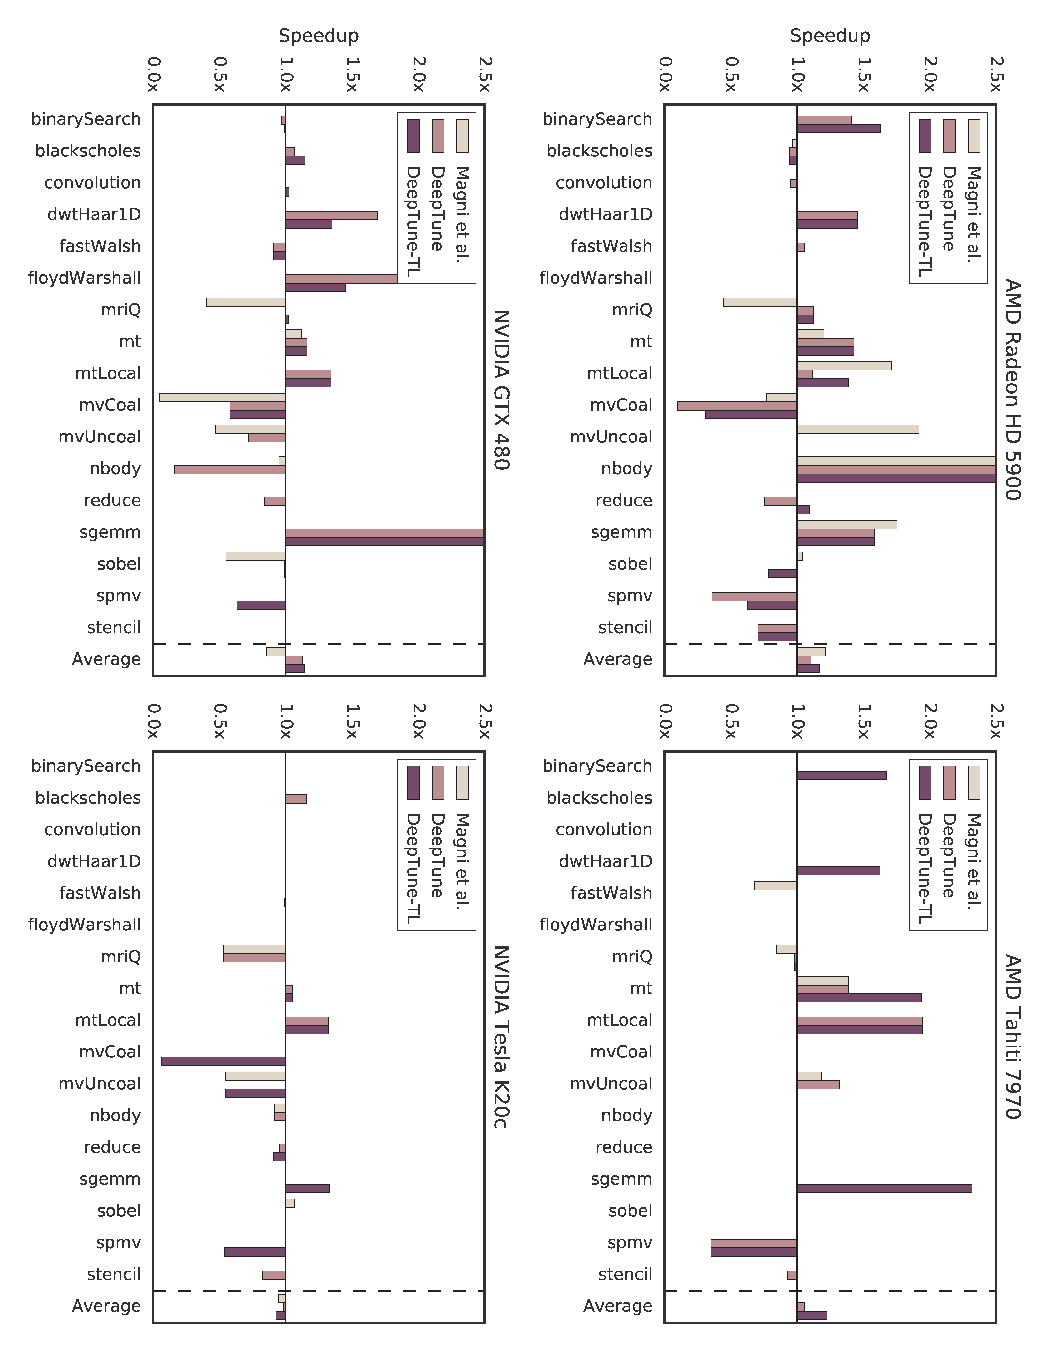
\includegraphics[width=\textwidth]{img/pact-speedup}%
	\caption[Speedups of predicted thread coarsening factors]{%
		Speedups of predicted coarsening factors for each platform. DeepTune outperforms \citeauthor{Magni2014}on three of the four platforms. Transfer learning improves DeepTune speedups further, by 16\% on average.%
	}%
	\label{fig:pact-speedup}
\end{figure}

On the NVIDIA Tesla K20c, the platform for which no predictive model achieves positive average speedups, DeepTune-TL matches or improve performance in the majority of cases, but over-coarsening on three of the programs causes a modest reduction in average performance. For this platform, further performance results are suspected necessary due to its unusual optimisation profile.


\section{DeepTune Internal Activation States}
\label{sec:deeptune-internal-states}

In previous sections DeepTune is shown to automatically outperform state-of-the-art predictive models for which experts have invested a great amount of time in engineering features. This section attempts to illuminate the inner workings, using a single example from Case Study B: predicting the thread coarsening factor for Parboil's \texttt{mriQ} benchmark on four different platforms.

Figure~\ref{fig:viz} shows the DeepTune configuration, with visual overlays showing the internal state. From top to bottom, the input to the model is the 267 lines of OpenCL code for the \texttt{mriQ} kernel. This source code is preprocessed, formatted, and rewritten using variable and function renaming, shown in Figure~\ref{fig:viz}b. The rewritten source code is tokenised and encoded in a $1$-of-$k$ vocabulary. Figure~\ref{fig:viz}c shows the first 80 elements of this encoded sequence as a heat map in which each cell's colour reflects its encoded value. The input, rewriting, and encoding is the same for each of the four platforms.

\begin{figure*}
  \centering %
  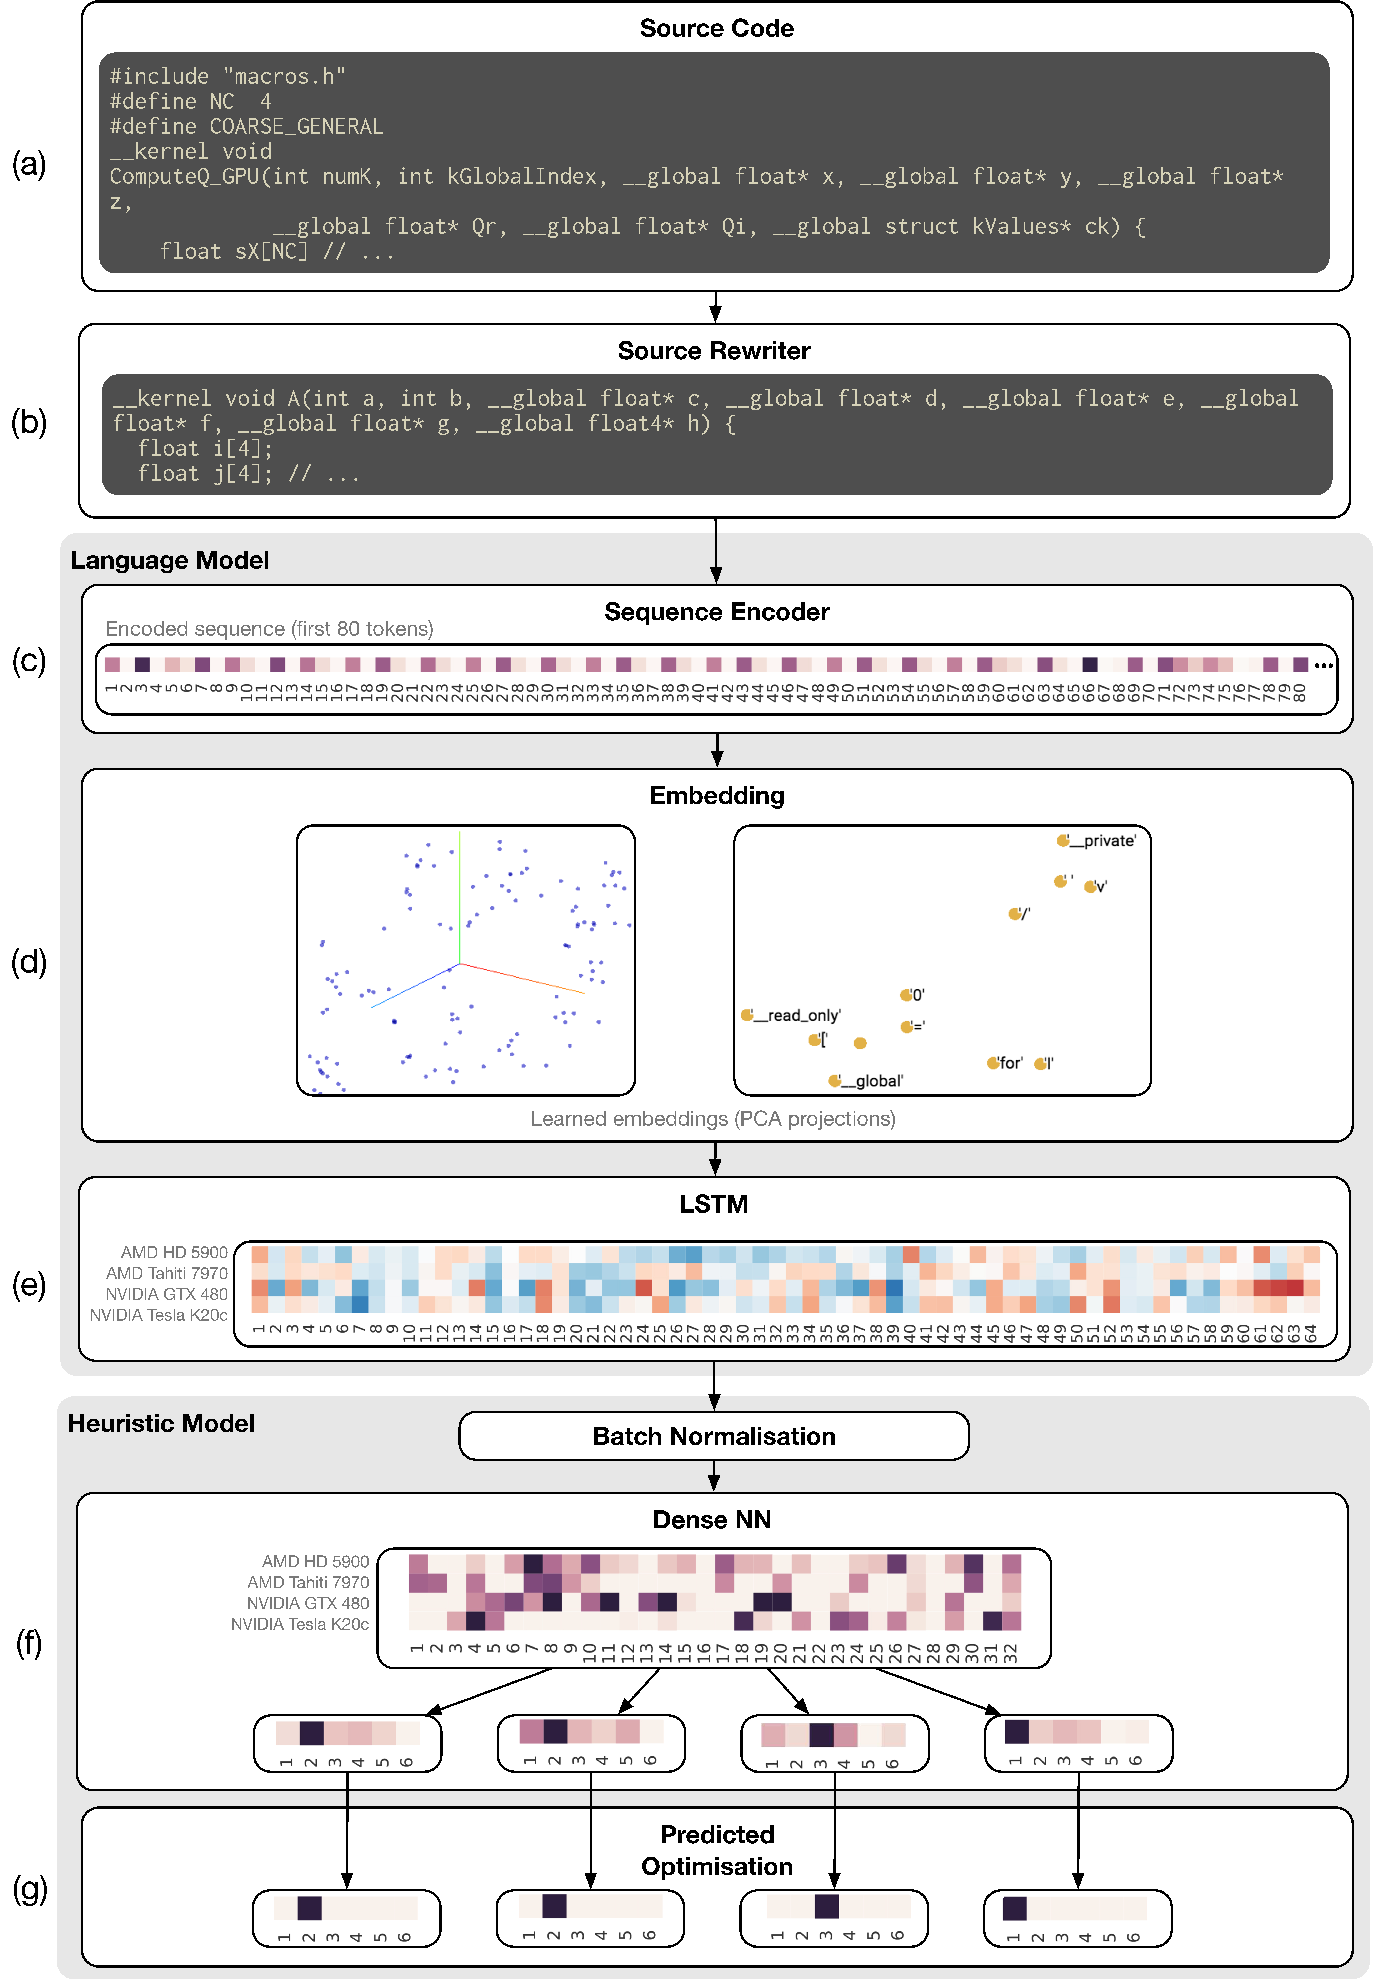
\includegraphics[width=\textwidth]{img/viz}%
    \vspace{-1em}
  \caption{%
    Visualizing the internal state of DeepTune when predicting coarsening factor
    for Parboil's \texttt{mriQ} benchmark on four different architectures. The
    activations in each layer of the four models increasingly diverge the lower
    down the network.%
  }
  \label{fig:viz} %
\end{figure*}


The encoded sequences are then passed into the Embedding layer. This maps each token of the vocabulary to a point in a 64 dimension vector space. Embeddings are learned during training so as to cluster semantically related tokens together. As such, they may differ between the four platforms. Figure~\ref{fig:viz}d shows a PCA projection of the embedding space for one of the platforms, showing multiple clusters of tokens. By honing in on one of the clusters and annotating each point with its corresponding token, it can be observed that the cluster contains the semantically related OpenCL address space modifiers \texttt{\_\_private}, \texttt{\_\_global}, and \texttt{\_\_read\_only}.

Two layers of 64 LSTM neurons model the sequence of embeddings, with the neuron activations of the second layer being used to characterise the entire sequence. Figure~\ref{fig:viz}e shows the neurons in this layer for each of the four platforms, using a red-blue heat map to visualise the intensity of each activation. Comparing the activations between the four platforms, we note a number of neurons in the layer with different responses across platforms. This indicates that the language model is partly specialised to the target platform. Subsequent experiments in~\cite{Ben-nun2018} support this reasoning, where a platform-agnostic language model achieves slightly poorer performance.

As information flows through the network, the layers become progressively more specialised to the specific platform. This can be seen in Figure~\ref{fig:viz}f, which shows the two layers of the heuristic model. The activations within these increasingly diverge. The mean variance of activations across platforms increases threefold compared to the language model, from 0.039 to 0.107. Even the activations of the AMD HD 5900 and AMD Tahiti 7970 platforms are dissimilar, despite the final predicted coarsening factor for both platforms being the same. The largest activation of the output layer is taken in Figure~\ref{fig:viz}g as the final predicted coarsening factor. For this particular program, a state-of-the-art model achieves 54\% of the maximum performance. DeepTune achieves 99\%.



%
%
%
%
%
%\section{Experimental Methodology}
%\label{sec:deeptune-methodology}
%
%DeepTune is applied to two heterogeneous compiler-based machine learning tasks and its performance compared to state-of-the-art approaches that use expert selected features.
%
%
%\subsection{Case Study A: OpenCL Heterogeneous Mapping}
%
%OpenCL provides a platform-agnostic framework for heterogeneous parallelism. This allows a program written in OpenCL to execute transparently across a range of different devices, from CPUs to GPUs and FPGAs. Given a program and a choice of execution devices, the question then is on which device should we execute the program to maximise performance?
%
%\subsubsection{State-of-the-art}
%
%In~\cite{Grewe2013}, \citeauthor{Grewe2013} develop a predictive model for mapping OpenCL kernels to the optimal device in CPU/GPU heterogeneous systems. They use supervised learning to construct decision trees, using a combination of static and dynamic kernel features. The static program features are extracted using a custom LLVM pass; the dynamic features are taken from the OpenCL runtime.
%
%\subsubsection{Expert Chosen Features}
%
%Table~\ref{tab:grewe-features-final} shows the features used by their work. Each feature is an expression built upon the code and runtime metrics given in Table~\ref{tab:grewe-features-raw}.
%
%\begin{table}
  \rowcolors{2}{gray!25}{white}
  \centering%
  \subfloat[Feature values]{
    \begin{tabular}{| l L{4.5cm} |}
      \hline
      \rowcolor{gray!50}
      \textbf{Name} & \textbf{Description} \\
      \hline
      \texttt{F1: data size/(comp+mem)} & commun.-computation ratio \\
      \texttt{F2: coalesced/mem} & \% coalesced memory accesses \\
      \texttt{F3: (localmem/mem)$\times$wgsize} & ratio local to global mem accesses  $\times$ \#.\ work-items \\
      \texttt{F4: comp/mem} & computation-mem ratio\\
      \hline
    \end{tabular}%
    \label{tab:grewe-features-final}%
  }\\ %
  \subfloat[Values used in feature computation]{%
    \rowcolors{2}{gray!25}{white}
    \begin{tabular}{| l c l |}
    	\hline
      \rowcolor{gray!50}
      \textbf{Name} & \textbf{Type} & \textbf{Description} \\
      \hline
      \texttt{comp} & static & \#.\ compute operations \\
      \texttt{mem} & static & \#.\ accesses to global memory \\
      \texttt{localmem} & static & \#.\ accesses to local memory \\
      \texttt{coalesced} & static & \#.\ coalesced memory accesses \\
      \texttt{data size} & dynamic & size of data transfers \\
      \texttt{work-group size} & dynamic & \#.\ work-items per kernel \\
      \hline
    \end{tabular}%
    \label{tab:grewe-features-raw}%
  }
  \caption[Heterogeneous mapping model features]{%
    Features used by \emph{Grewe et al. }to predict heterogeneous device
    mappings for OpenCL kernels.%
  } %
  \label{tab:grewe-features} %
\end{table}

%
%\subsubsection{Experimental Setup}
%
%The predictive model of \citeauthor{Grewe2013}~\cite{Grewe2013} is replicated. The same experimental setup is used as in Section~\ref{sec:clgen-eval-methodology} in which the experiments are extended to a larger set of 71 programs, summarised in Table~\ref{tab:cgo-benchmarks}. The programs were evaluated on two CPU-GPU platforms, detailed in Table~\ref{tab:cgo-platforms}.
%
%\begin{table}
\centering%
\rowcolors{2}{white}{gray!25}
\subfloat[Case Study A: OpenCL Heterogeneous Mapping]{%
  \begin{tabular}{l r r r}
    \toprule
    & \textbf{Version} & \textbf{\#. benchmarks} & \textbf{\#. kernels}\\
    \midrule
    \textbf{NPB (SNU~\cite{Seo2011})} & 1.0.3 & 7 & 114 \\
    \textbf{Rodinia~\cite{Che2009}} & 3.1 & 14 & 31 \\
    \textbf{NVIDIA SDK} & 4.2 & 6 & 12 \\
    \textbf{AMD SDK} & 3.0 & 12 & 16 \\
    \textbf{Parboil~\cite{Stratton2012}} & 0.2 & 6 & 8 \\
    \textbf{PolyBench~\cite{Grauer-Gray2012}} & 1.0 & 14 & 27 \\
    \textbf{SHOC~\cite{Danalis2010}} & 1.1.5 & 12 & 48 \\
    \textbf{Total} & - & 71 & 256 \\
    \bottomrule
  \end{tabular}
  \label{tab:cgo-benchmarks}
}\\*
\subfloat[Case Study B: OpenCL Thread Coarsening Factor]{%
  \begin{tabular}{l r r r}
    \toprule
    & \textbf{Version} & \textbf{\#. benchmarks} & \textbf{\#. kernels}\\
    \midrule
    \textbf{NVIDIA SDK} & 4.2 & 3 & 3 \\
    \textbf{AMD SDK} & 3.0 & 10 & 10 \\
    \textbf{Parboil~\cite{Stratton2012}} & 0.2 & 4 & 4 \\
    \textbf{Total} & - & 17 & 17 \\
    \bottomrule
  \end{tabular}
  \label{tab:pact-benchmarks}
}\\*
\caption{Benchmark programs.} %
\label{tab:benchmarks} %
\end{table}

%\begin{table}[t!]
  \centering %
  \subfloat[Case Study A: OpenCL Heterogeneous Mapping]{%
  \rowcolors{2}{gray!25}{white}
  \begin{tabular}{| l l l l| }
    \hline
    \rowcolor{gray!50}
    & \textbf{Frequency} & \textbf{Memory} & \textbf{Driver} \\
    \hline
    \textbf{Intel Core i7-3820} & 3.6 GHz & 8GB & AMD 1526.3 \\
    \textbf{AMD Tahiti 7970} & 1000 MHz & 3GB & AMD 1526.3 \\
    \textbf{NVIDIA GTX 970} & 1050 MHz & 4GB & NVIDIA 361.42 \\
    \hline
  \end{tabular}
  \label{tab:cgo-platforms}
  }\\*
  \subfloat[Case Study B: OpenCL Thread Coarsening Factor]{%
  \rowcolors{2}{gray!25}{white}
  \begin{tabular}{| l l l l |}
    \hline
    \rowcolor{gray!50}
    & \textbf{Frequency} & \textbf{Memory} & \textbf{Driver} \\
    \hline
    \textbf{AMD HD 5900} & 725 MHz & 2GB & AMD 1124.2 \\
    \textbf{AMD Tahiti 7970} & 1000 MHz & 3GB & AMD 1084.4 \\
    \textbf{NVIDIA GTX 480} & 700 MHz & 1536 MB & NVIDIA 304.54 \\
    \textbf{NVIDIA K20c} & 706 MHz & 5GB & NVIDIA 331.20 \\
    \hline
  \end{tabular}
  \label{tab:pact-platforms}
  }
  \caption{Experimental platforms.}
  \label{tab:platforms}
\end{table}

%
%\subsubsection{DeepTune Configuration}
%
%Figure~\ref{fig:nn}a shows the neural network configuration of DeepTune for the task of predicting optimal device mapping. The OpenCL kernel source code is used as input, along with the two dynamic values \emph{work-group size} and \emph{data size} available to the OpenCL runtime.
%
%\subsubsection{Model Evaluation}
%
%\emph{Stratified 10-fold cross-validation} is used to evaluate the quality of the predictive models~\cite{Han2011}. Each program is randomly allocated into one of 10 equally-sized sets; the sets are balanced to maintain a distribution of instances from each class consistent with the full set. A model is trained on the programs from all but one of the sets, then tested on the programs of the unseen set. This process is repeated for each of the 10 sets, to construct a complete prediction over the whole data set.
%
%\begin{figure}[t!]
  \centering
  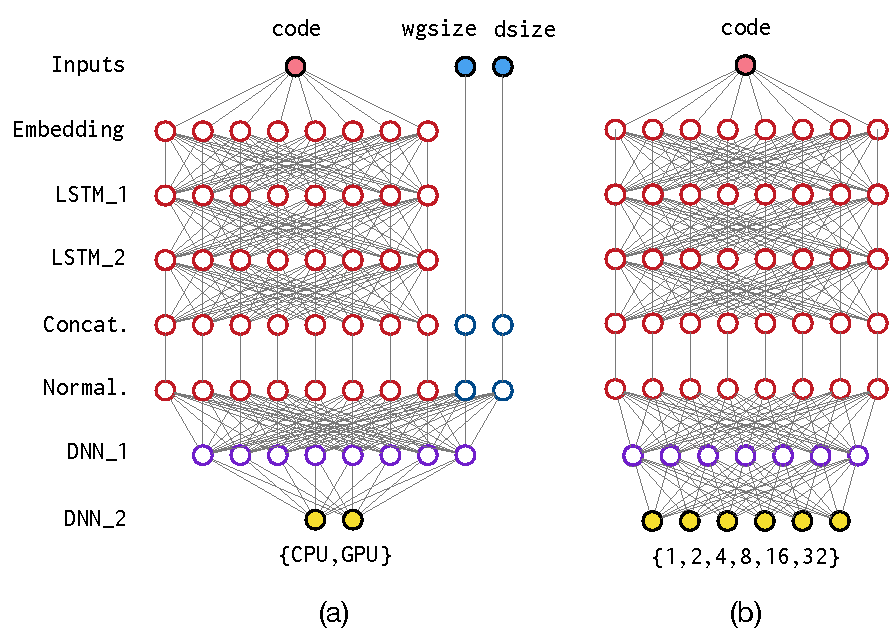
\includegraphics[width=\columnwidth]{img/nn} %
  \caption[DeepTune artificial neural networks]{%
    DeepTune artificial neural networks, configured for (a) heterogeneous mapping, and (b) thread coarsening factor. The design stays almost the same regardless of the optimisation problem. The only changes are the extra input for (a) and size of the output layers.%
  }%
  \label{fig:nn}
\end{figure}

%
%
%\subsection{Case Study B: OpenCL Thread Coarsening Factor}
%
%Thread coarsening is an optimisation for parallel programs in which the operations of two or more threads are fused together. This optimisation can prove beneficial on certain combinations of programs and architectures, for example programs with a large potential for Instruction Level Parallelism on Very Long Instruction Word architectures.
%
%\subsubsection{State-of-the-art} \citeauthor{Magni2014}present a predictive model for OpenCL thread coarsening in~\cite{Magni2014}. They implement an iterative heuristic which determines whether a given program would benefit from coarsening. If yes, then the program is coarsened, and the process repeats, allowing further coarsening. In this manner, the problem is reduced from a multi-label classification problem into a series of binary decisions, shown in Figure~\ref{fig:cf-magni}. They select from one of six possible coarsening factors: $(1, 2, 4, 8, 16, 32)$, divided into 5 binary choices.
%
%\begin{figure}
  \centering %
  \subfloat[Magni \emph{et al.\ }cascading binary model.]{%
    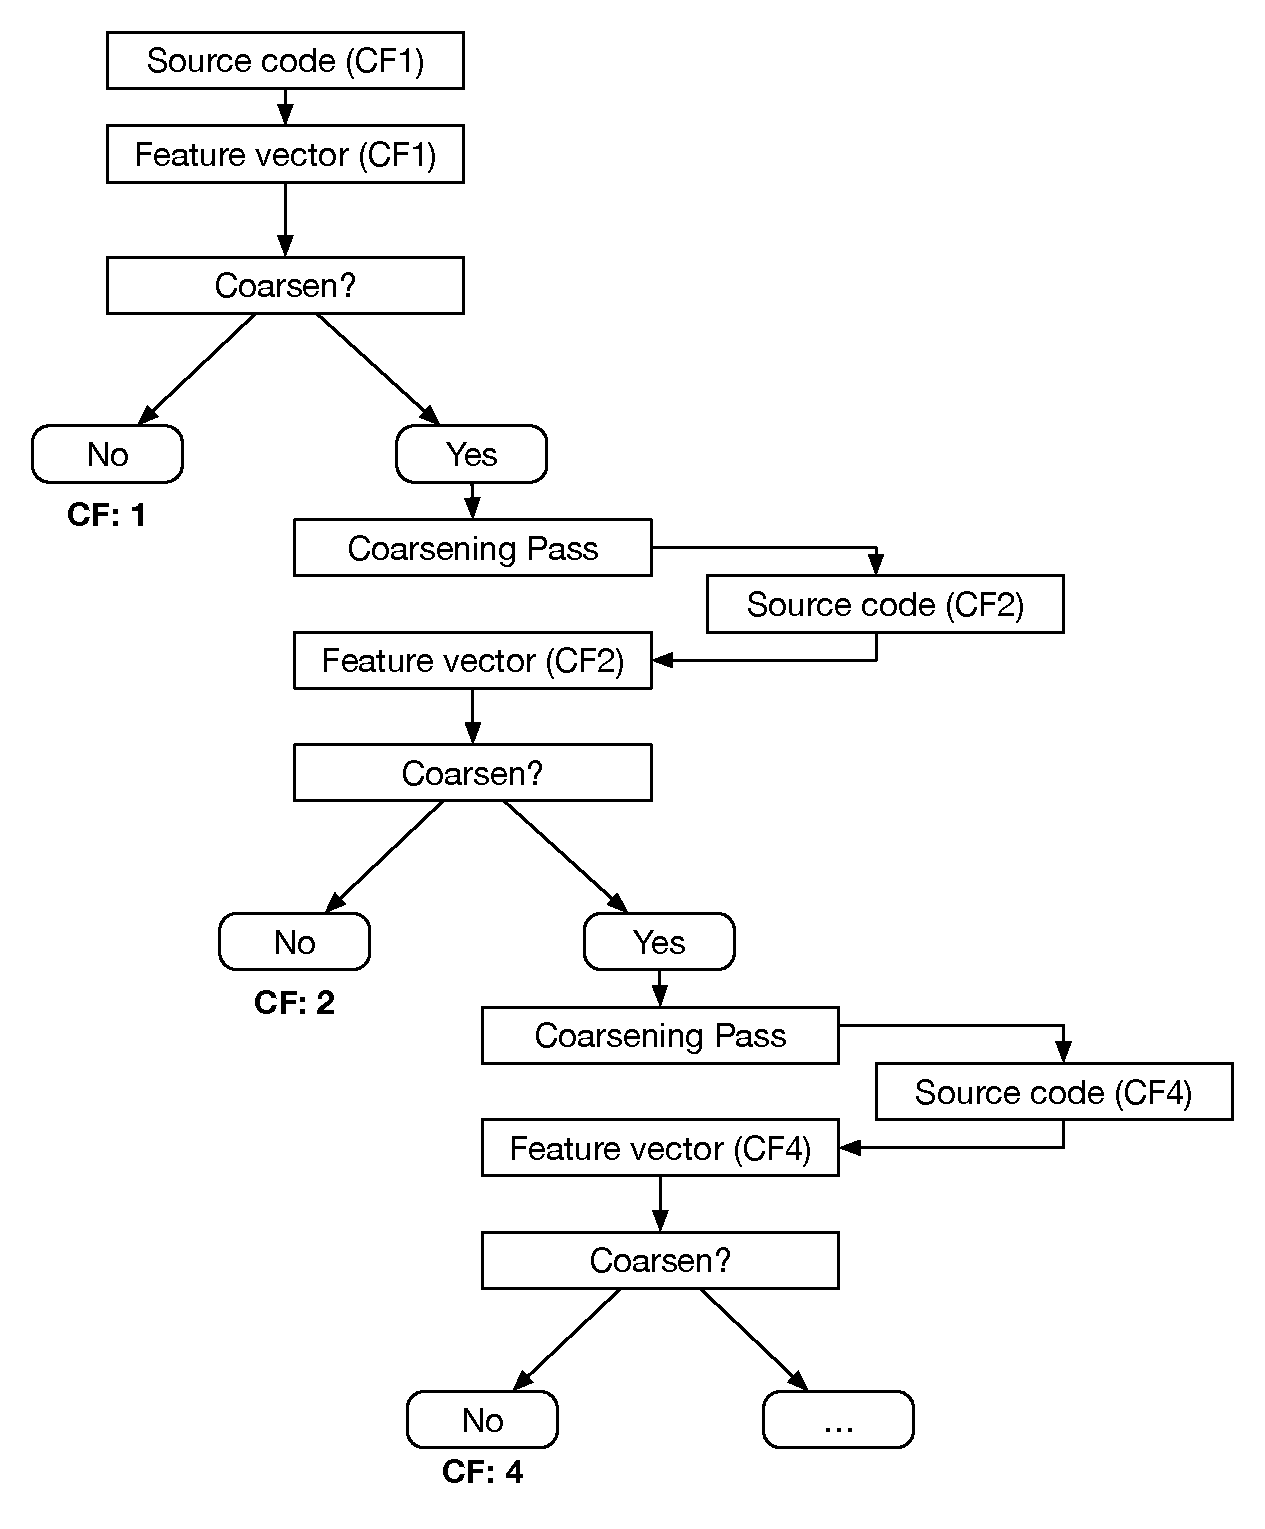
\includegraphics[width=.85\columnwidth]{img/cf-magni}%
    \label{fig:cf-magni}
  }\\*%
  \subfloat[Our approach.]{%
      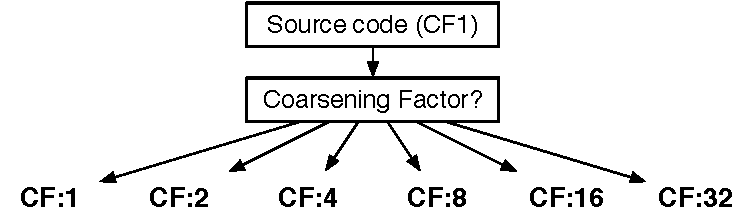
\includegraphics[width=.65\columnwidth]{img/cf-deeptune}%
      \label{fig:cf-deeptune}
  }%
  \caption{%
      Two approaches for predicting coarsening factor (CF) of OpenCL kernels.
      Magni \emph{et al.\ }reduce the multi-label classification problem to a
      series of binary decisions, by iteratively applying the optimization and
      computing new feature vectors. Our approach simply predicts the coarsening
      factor directly from the source code.%
  }
  \label{fig:cascading-nn}
\end{figure}

%
%\begin{table}
  \rowcolors{2}{gray!25}{white}
  \centering%
    \begin{tabular}{| l l |}
      \hline
      \rowcolor{gray!50}
      \textbf{Name} & \textbf{Description} \\
      \hline
      \texttt{BasicBlocks} & \#.\ basic blocks \\
      \texttt{Branches} & \#.\ branches \\
      \texttt{DivInsts} & \#.\ divergent instructions \\
      \texttt{DivRegionInsts} & \#.\ instructions in divergent regions \\
      \texttt{DivRegionInstsRatio} & \#.\ instr. in divergent regions / total instructions \\
      \texttt{DivRegions} & \#.\ divergent regions \\
      \texttt{TotInsts} & \#.\ instructions \\
      \texttt{FPInsts} & \#.\ floating point instructions \\
      \texttt{ILP} & average ILP / basic block \\
      \texttt{Int/FP Inst Ratio} & \#.\ branches \\
      \texttt{IntInsts} & \#.\ integer instructions \\
      \texttt{MathFunctions} & \#.\ match builtin functions \\
      \texttt{MLP} & average MLP / basic block \\
      \texttt{Loads} & \#.\ loads \\
      \texttt{Stores} & \#.\ stores \\
      \texttt{UniformLoads} & \#.\ loads unaffected by coarsening direction \\
      \texttt{Barriers} & \#.\ barriers \\
      \hline
    \end{tabular}%
    \label{tab:features-pact14-raw}%
  \caption[\emph{Magni et al.\ }features for predicting thread coarsening]{%
    Candidate features used by \emph{Magni et al.\ }for predicting thread
    coarsening. From these values, they compute relative deltas for each
    iteration of coarsening, then use PCA for selection.%
  }%
  \label{tab:magni-features} %
\end{table}

%
%\subsubsection{Expert Chosen Features}
%
%\citeauthor{Magni2014}followed a very comprehensive feature engineering process. 17 candidate features were assembled from previous studies of performance counters and computed theoretical values~\cite{Magni2,Sim2012}. For each candidate feature they compute its coarsening \emph{delta}, reflecting the change in each feature value caused by coarsening: $f_{\Delta} = (f_{after} - f_{before}) / f_{before}$, adding it to the feature set. Then they use Principle Component Analysis (PCA) on the 34 candidates and selected the first 7 principle components, accounting for 95\% of variance in the space.
%
%\subsubsection{Experimental Setup}
%
%The experimental setup of \citeauthor{Magni2014}~\cite{Magni2014} is replicated. The thread coarsening optimisation is evaluated on 17 programs, listed in Table~\ref{tab:pact-benchmarks}. Four different GPU architectures are used, listed in Table~\ref{tab:pact-platforms}.
%
%\subsubsection{DeepTune Configuration}
%
%Figure~\ref{fig:nn}b shows the neural network configuration. The OpenCL kernel is the sole input the coarsening factor is the predicted output.
%
%\subsubsection{Model Evaluation}
%
%Compared to Case Study A, the size of the evaluation is small. We use \emph{leave-one-out cross-validation} to evaluate the models. For each program, a model is trained on data from all other programs and used to predict the coarsening factor of the excluded program.
%
%The parameters of the neural network is not described in~\cite{Magni2014}, so an additional, \emph{nested} cross-validation process is used to find the optimal model parameters. For every program in the training set, 48 combinations of network parameters are evaluated. The best performing configuration is selected from these 768 results to train a model for prediction on the excluded program. This nested cross-validation is repeated for each of the training sets. No such tuning of hyper-parameters is performed for DeepTune.
%
%
%\subsection{Comparison of Case Studies}
%
%For the two different optimisation heuristics, the authors arrived at very different predictive model designs, with very different features. By contrast, the DeepSmith approach is exactly the same for both problems. None of DeepTune's parameters were tuned for the case studies presented above. Their settings represent conservative choices expected to work reasonably well for most scenarios.
%
%Table~\ref{tab:nn-size} shows the similarity of the models. The only difference between the network designs is the auxiliary inputs for Case Study A and the different number of optimisation decisions. The differences between DeepTune configurations is only two lines of code: the first, adding the two auxiliary inputs; the second, increasing the size of the output layer for Case Study B from two neurons to six. The description of these differences is larger than the differences themselves.
%
%\begin{table}
  \centering
  \rowcolors{2}{white}{gray!25}
  \begin{tabular}{| l r r | r r |}
    \hline
    \rowcolor{gray!50}
    & \multicolumn{2}{c}{\textbf{\#.\ neurons}} & \multicolumn{2}{c}{\textbf{\#.\ parameters}} \\
    \rowcolor{gray!50}
    & \textbf{HM} & \textbf{CF} & \textbf{HM} & \textbf{CF} \\
    \hline
    \textbf{Embedding} & 64 & 64 & ,256 & 8,256 \\
    \textbf{LSTM\_1} & 64 & 64 & 33,024 & 33,024 \\
    \textbf{LSTM\_2} & 64 & 64 & 33,024 & 33,024 \\
    \textbf{Concatenate} & 64 + 2 & - & - & - \\
    \textbf{Batch Normalisation} & 66 & 64 & 264 & 256 \\
    \textbf{DNN\_1} & 32 & 32 & 2,144 & 2,080 \\
    \textbf{DNN\_2} & 2 & 6 & 66 & 198 \\
    \hline
    \textbf{Total} & & & 76,778 & 76,838 \\
    \hline
  \end{tabular}
  \caption[DeepTune model parameters]{%
    The size and number of parameters of the DeepTune components of
    Figure~\ref{fig:nn}, configured for heterogeneous mapping (HM) and
    coarsening factor (CF).%
  }
  \label{tab:nn-size}
\end{table}

